\chapter{Design Procedures}

To create the NIRS system, a sensor consisting of LEDs, to emit light through the area of interest, and photodiodes, to convert the transmitted incident light into an electrical signal, must be made. The signal from the photodiodes must then be connected to an ADC in order to convert the analog signal to a digital signal that is readable by the computer doing the calculations. The digital signal must then be transmitted to the computer where calculations would be done.

To control the LEDs and convert the analog signal to a digital one, a microcontroller will be used. The microcontroller will then be interfaced to a computer through UART, initially through USB, then finally wirelessly through Bluetooth. The overall system can be seen in Figure 4.1.

\begin{figure}[htp]
\centering
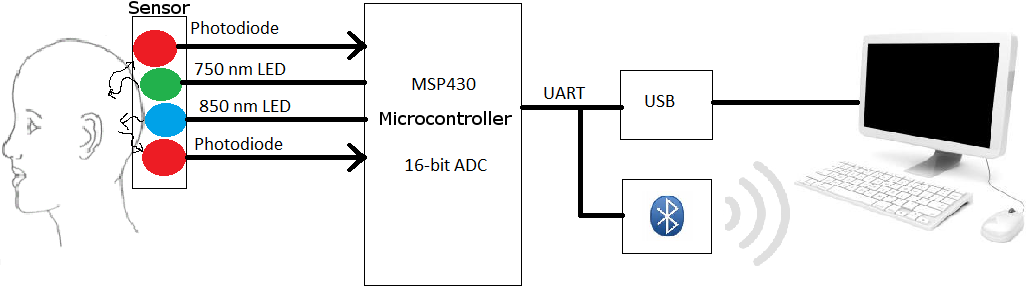
\includegraphics[width=6in]{design.png}
\caption[A very basic overview of the system.]{A very basic overview of the system. For the testing phase, USB will be used to communicate with the computer. Eventually, Bluetooth will be used as the primary means of communication.}
\end{figure}

Bluetooth was selected over a low power wireless interface, such as ZigBee, due to Bluetooth being widely available on all modern phones. It was the intention to interface the device with a mobile phone, time permitting. However, this was never done. Bluetooth consumes much more power than other competing wireless communication systems, so to obtain optimum battery life it is not ideal. Had the author realized that there would be no time to interface the device with a mobile phone, a lower power wireless communication system would have been selected, most probably ZigBee.

To design the NIRS system, it was decided to design everything from scratch. The microcontroller circuit, the sensor, as well as the software was designed and built/written. This was done to truly test the author's knowledge obtained from his years at McMaster University. Additionally, this project provided an excellent chance to be introduced to microcontroller circuit design.

Development of this system began with the microcontroller, since nothing would work without it, followed by the sensor, then finally the software.

\section{The Microcontroller}

The microcontroller selected for use in this project is the Texas Instruments MSP430, specifically the MSP430f4250. The MSP430 was chosen due to its low power requirements and 16-bit sigma-delta ADC. In most cases, a 12-bit ADC would be sufficient, but a higher resolution will allow for the weak temporal signals to be detected easier. The MSP430 is also fairly cheap. These characteristics make it ideal for this project and made it standout from other competitors. 

While the MSP430f4250 is slightly excessive for this project, due to its built in LCD controller and array of I/O ports, it was the cheapest MSP430 model that the minimum required I/O ports and a 16-bit ADC.

While the MSP430f4250 does not have any dedicated UART hardware on-board, a software timer UART is sufficient in this project. The project only requires samples to be transmitted from the microcontroller to a computer. It was decided that flow control was not necessary for this project. This decision, however, led to many problems during testing, which will be discussed later. 

To design the microcontroller circuit, datasheets, user guides, application notes, and reference designs were read and used as a basis. Thankfully, the MSP430 has many built in capacitors and resistors (for example, adjustable oscillator capacitors) that help to reduce the overall components of the  build. The schematic of the device can be seen in Figure 4.2

\begin{figure}[htp]
\centering
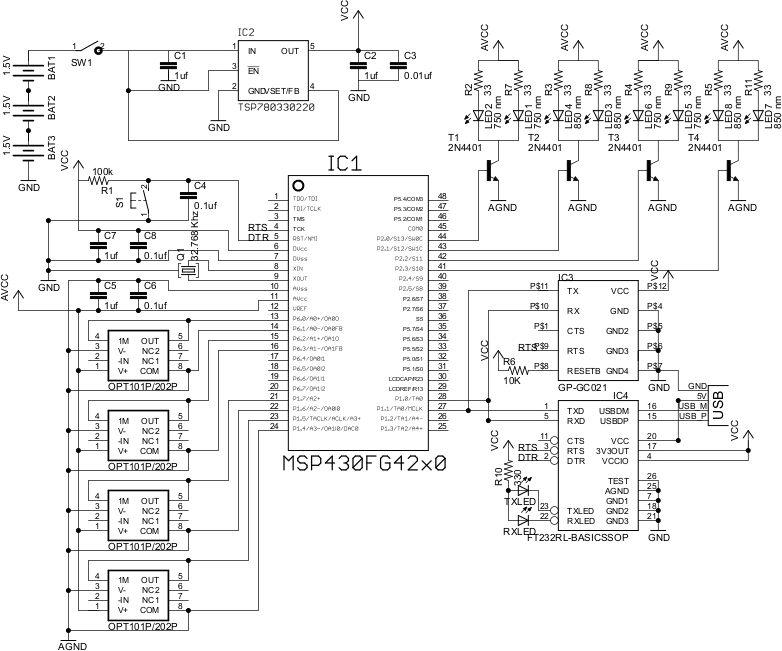
\includegraphics[width=6in]{mcu.png}
\caption[Schematic of the system]{The schematic of the overall system. Note that two sensors are included in the diagram. The TPS79433 LDO regulator was used instead of the TPS780330220 in the diagram}
\end{figure}

A 32.768 Khz crystal is used because that is the only crystal the MSP430f4250 is designed to use. It is used as somewhat as a watchdog timer, waking the MSP430 up at select intervals to see if there is work to be done, unless it is told otherwise. Capacitors between VCC and GND were placed as close the the microcontroller as possible, as per Dr. Doyle's suggestion. This helps to reduce any noise that may have been picked up between the power supply and the microcontroller. This is especially a problem with the MSP430, any fluctuations/noise in the power supplied to it will cause the ADC to be very noisy. This is perhaps the main reason why the MSP430 is not very popular in projects that require signal acquisition. However, with proper consideration, this should not be much of an issue. To further reduce the noise in the ADC, separate power and ground are used for digital signals and analog signals, VCC \& GND and AVCC \& AGND respectively. 

The frequency the microcontroller operates at is governed by the voltage supplied by its power supply. Since the Bluetooth module operates at 3.3V and the USB UART device outputs power at 3.3V when powered by USB, a 3.3V power supply was selected. This sets the frequency of the microcontroller to ~7 Mhz, which is set by a FLL (frequency-locked loop). The speed the microcontroller operates at is of no big importance in this project. The sampling rate for data acquisition is slow enough, at 100Hz, that the 32Khz crystal is fast enough to supply the clock at which to sample the data. The speed of the UART is what is affected by the microcontroller speed. It was determined that the speed of the UART must be at least 76 800 bit/s or 76.8k baud (see Appendix A), which is easily exceed with a clock ~7Mhz.

To supply this voltage, 3 AA batteries connected to a regulator were chosen for long battery life. An LDO (low-dropout) regulator was selected over a more traditional regulator, such as an LM317. An LDO regulator was chosen because LDO regulators are highly efficient, consume very little power, and have low quiescent current, increasing battery life. Due to the the low power-requirements of every component, not much current is required by the system, making an LDO regulator ideal for use. LDO regulators are limited to the amount of current they can output due to consuming very little power.

The LDO regulator selected to do the job is the Texas Instruments TPS79433. It outputs voltages at 3.3V at a maximum current of 250mA. Additionally, it can be supplied power at less than 3.3V and will still output power at 3.3V. This is a nice feature because when the batteries drain to below 3.3V, the unit will still be operational. This regulator was selected because it meets all the requirements and free samples were obtainable from Texas Instruments. The circuit for the power supply was derived from the datasheet. 

To interface with the computer, the an USB to UART device was used. The FTDI FT232 was selected due to many good reviews on the device and good compatibility with Linux and Windows. The circuit design is based on the reference design given in the datasheet. One thing to note is that, while the built-in bootloader implemented flow control, which was necessary to invoke the bootloader, the software UART used in this project did not. As such, the DTR wire had to be disconnected from the microcontroller when not programming the device. Otherwise, the DTR wire would reset the device when communicating with the computer. The USB UART interface was used to program the device and initially communicate to the device during testing.

Once everything was deemed working, the Bluetooth module was added to interface with the computer. The Bluetooth module selected was RF-BTMX417 by MDFLY. This was selected due to its cheap price, Bluetooth 2.0 specifications, and low power requirements. The design for the Bluetooth module was based on the reference design in the datasheet.

Once all the parts were selected, the majority of the necessary parts were ordered from Digikey due to their cheap prices. Free samples were obtained of the microcontroller and LDO regulator from Texas Instruments. The Bluetooth module was ordered from ebay. The prototype was built on a breadboard using SMD to DIP adaptors for each component needing one. The prototype can be seen in figure 4.3

\begin{figure}[htp]
\centering
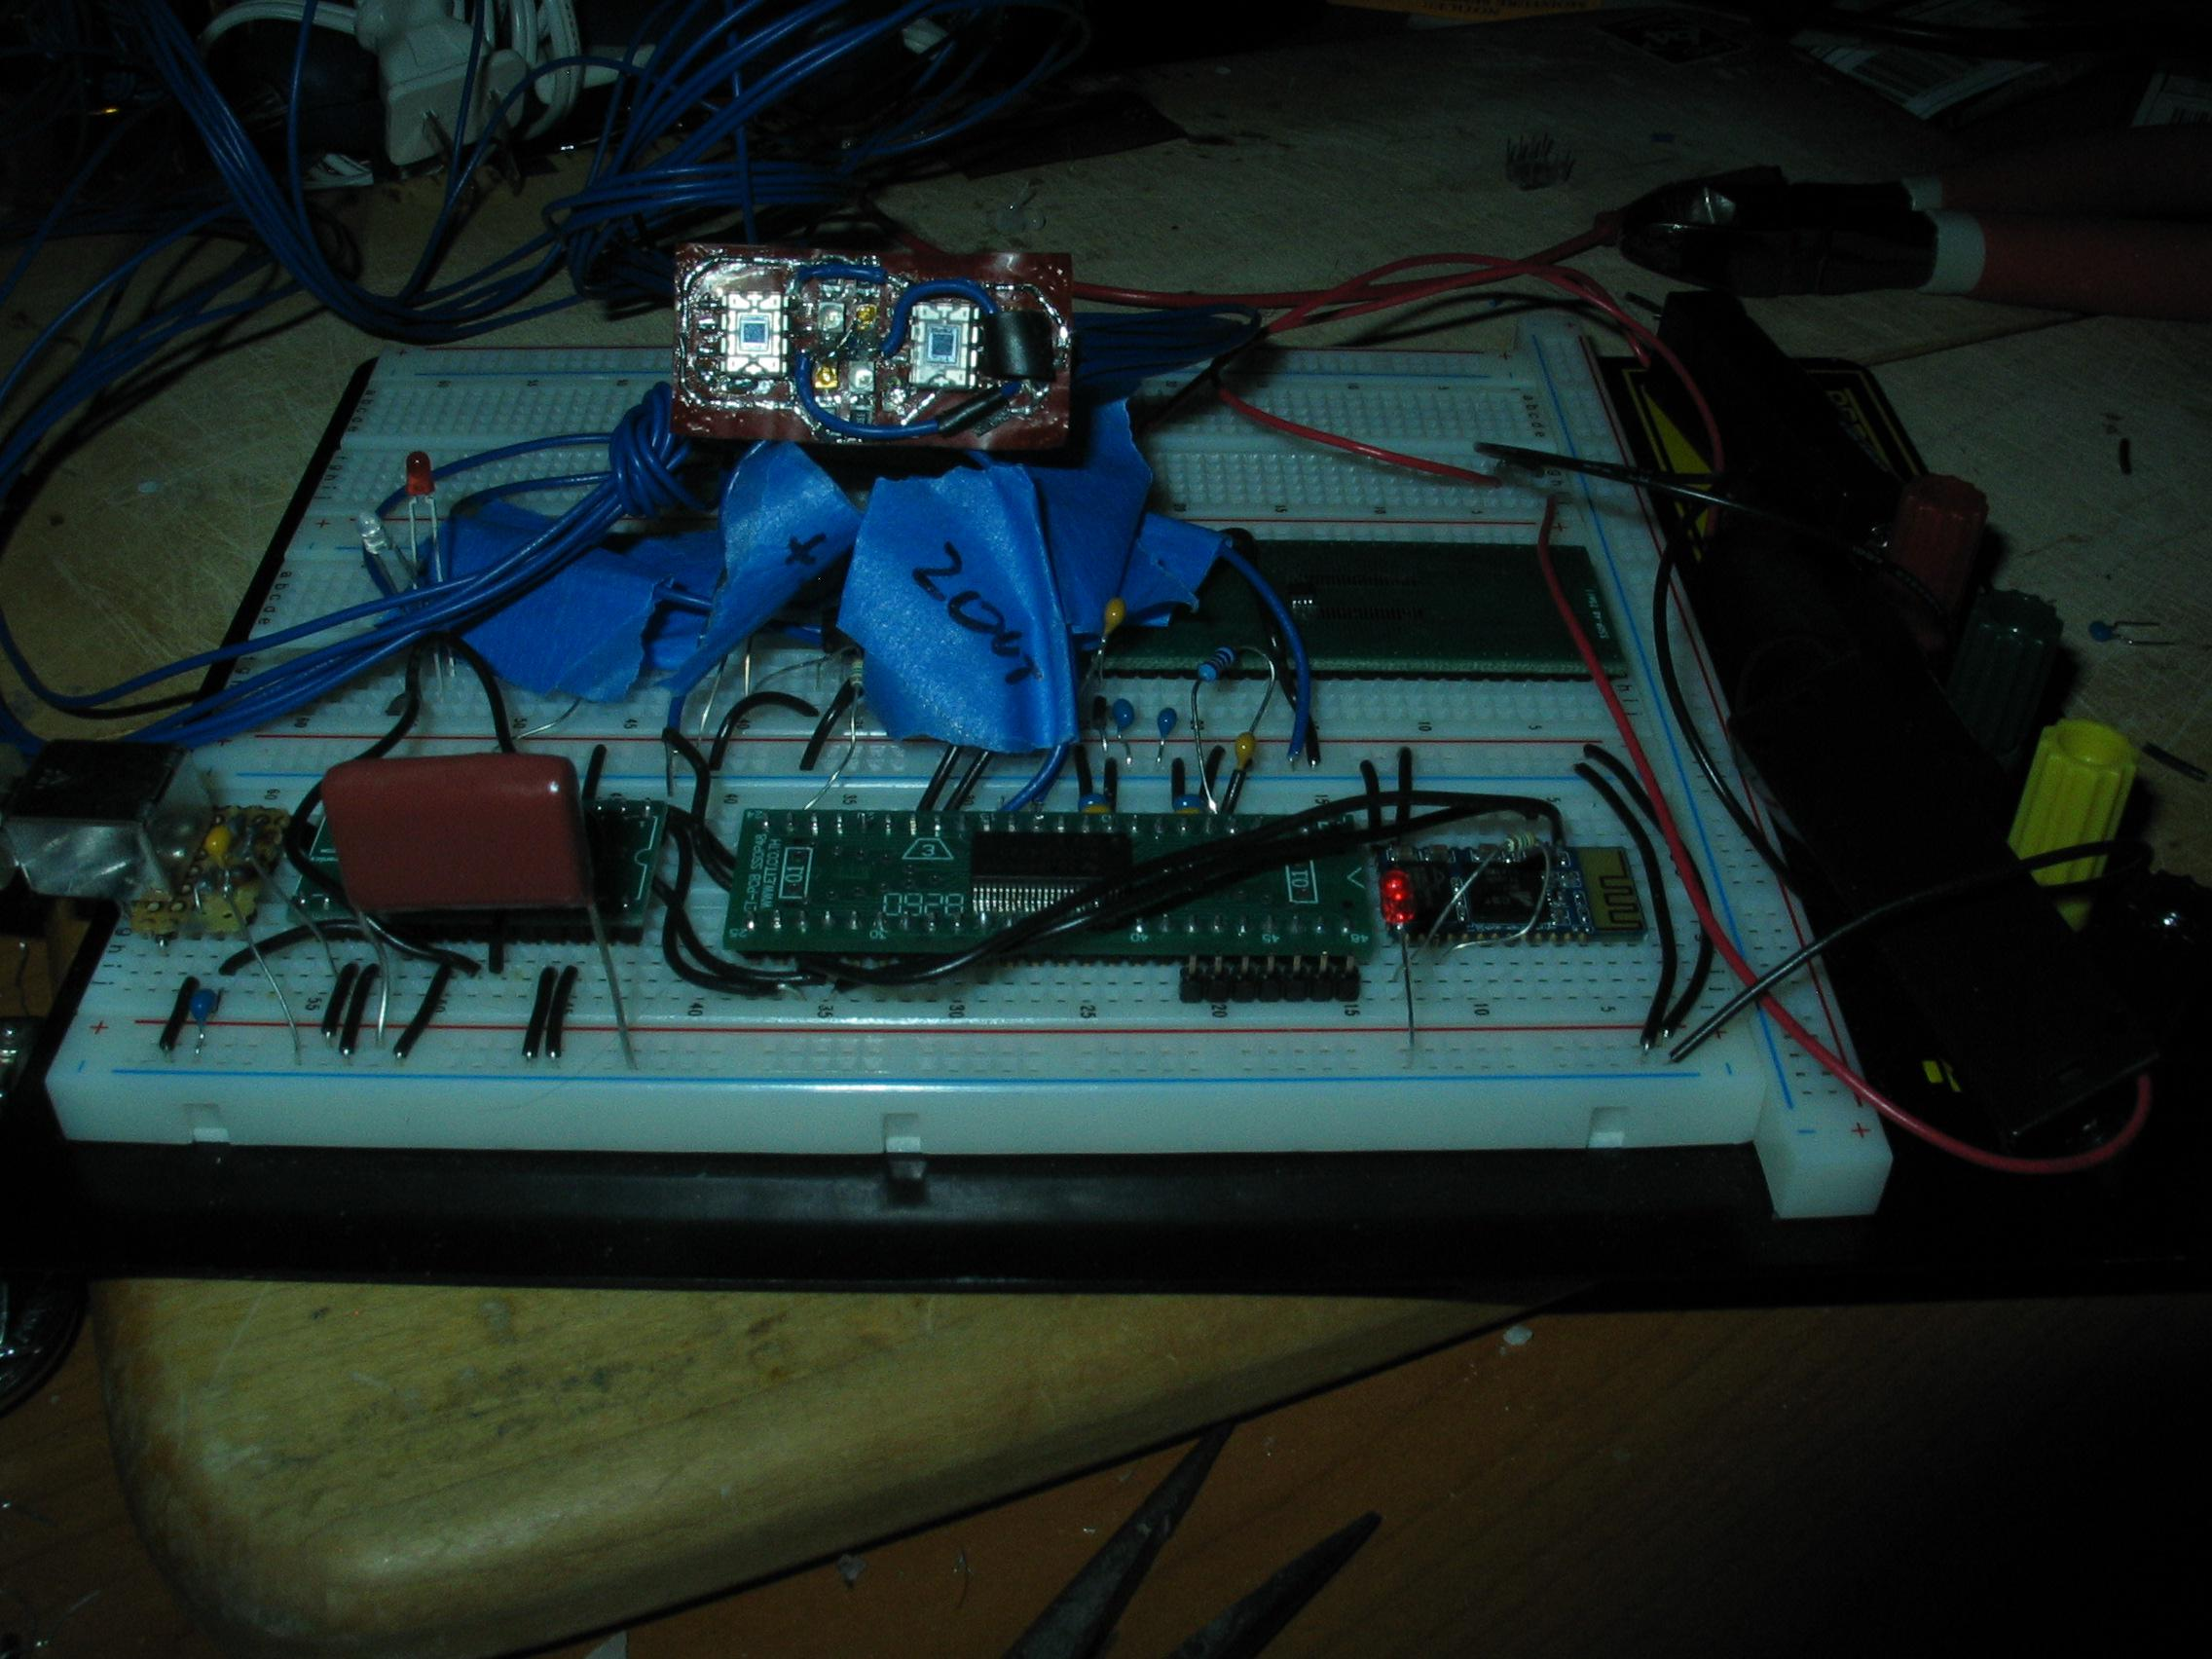
\includegraphics[width=6in]{prototype.jpg}
\caption[The Prototype]{Picture of the prototype}
\end{figure}


To program the device, the MSP430f4250 has a a built-in non-overwritable (without JTAG) bootloader that can be programming over UART. A JTAG programmer would have cost at least \$100, greatly increasing the cost of this project, though making debugging much easier. The mspgcc tools included software, written by developers at TinyOS, to write to the bootloader on the MSP430. The mspgcc toolchain was used to compile the software, specifically mspgcc-4.4.3, and then programed to the device using the TinyOS software.

\section{The Sensor}

The sensor was first designed by selecting the components. The main problem was sourcing the LEDs with the desired wavelengths. After many emails to various distributors and manufactures, it was discovered Marubeni Corporation sold 750nm SMD LEDs in low quantities. The epitex SMT750-25 to be exact. As such, 750 nm LEDs were selected as one light source.

The wavelength of the other LED light source, must be above 800nm and be such that it minimizes interference between the two LEDs. Based on the study done in [4], the LEDs with wavelengths of 750nm and 850nm were selected to minimize interference between each LED. The 750nm wavelength responds better to deoxygenation in the blood and the 850nm wavelength responds better to oxygenation in the blood. Luckily enough, the 850nm LEDs were easily sourceable from Digikey in SMD form. The OSRAM SFH4650 being the only 850nm LED easily obtainable, or rather only 800 - 870nm SMD LED easily obtainable. The OSRAM SFH4650 has very recently been replaced by the more efficient SFH4651, while still providing similar specifications.

Unfortunately, the spectral half width of the LEDs are broader than desired. The 750nm LEDs have a spectral half-width of $\pm$ 35nm. While the 850nm LEDs have a spectral half-width of $\pm$ 42nm. This means the effective wavelength may vary by the spectral half-width, causing cross-talk between the LEDs and possibly throwing off the calculations. They have narrow halfangles, however, $\pm$ 25$^\circ$ and $\pm$ 20$^\circ$, respectively, which is desired to limit light leakage and force the highest light intensity towards the area of interest. With a forward current of 100mA, it is assumed the approximate penetration depth of these LEDs is 1cm, based on past studies \cite{rosen05}.

The LEDs are the most power-hungry device in this system. They could not be directly driven by the microcontroller. NPN transistors were selected to do this task. Specifically, the 2N4401 600mA NPN general purpose transistor. The 2N4401 was selected as it was the cheapest transistor available at Digikey with greater than 200mA continuous collector current. Each led has a maximum forward current of 100mA, so to power the LEDs at their maximum intensity, a 200mA transistor would be needed. The microcontroller would turn the NPN transistor on when it was desired to turn its subsequent LED on. Setting the Base of the NPN transistor to high, would allow current to flow from the Collector to the Emitter. Setting the Base to low (GND), would stop the current from flowing from the collector to the emitter. For a high integration density, each sensor and each transistor would have 2 LEDs of the same wavelength. This can be seen in Figure 4.4.

\begin{figure}[htp]
\centering
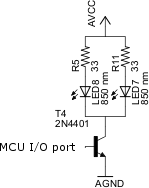
\includegraphics{led.png}
\caption[LED control diagram]{The schematic of controlling one wavelength of LED on the sensor}
\end{figure}

To detect the reflected light back, a photodiode must be used. However, the electrical signal measured by a photodiode varies in current, opposed to voltage as most ADCs work. As such, the current must be converted into corresponding voltage by a transimpedance amplifier. An interesting solution to this problem is the OPT101 by Burr-Brown. It is a monolithic photodiode with a built-in transimpedance amplifier, all in a small DIP-8 package. This makes it ideal for this project. Two photodiodes are placed on each sensor to pick up scattering and increase the overall surface area of the detectors.

The overall design of the sensor can be seen in Figure 4.5. It was decided that the transistors would be put on the PCB rather than on the sensor to reduce the size of the sensor.

\begin{figure}[htp]
\centering
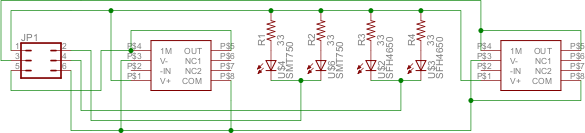
\includegraphics[width=6in]{sensor.png}
\caption[Sensor schematic]{The schematic of one sensor.}
\end{figure}

\subsection {Building the sensor}

Building the sensor was a daunting and hard task. The sensor had to be flexible to adhere to the head of the patient. As such, a flexible PCB is desired over a ridged one. 

To create the flexible PCB, the toner transfer method of homemade PCB creation was used. The PCB mill in the IEEE student Branch is not able to mill such a thin layer of copper on a flexible surface, and especially not with such thin tracings. 

The basic idea behind the toner transfer method is to print the design onto glossy paper using a laser printer. Melt the toner onto the copper board using an iron or something equally hot. Then etch the board using an enchant such as Ferric Chloride. Then to remove the toner from the PCB using a solvent such as acetone.

Dupont generously supplied a sample of dual sided Pyralux Copper PCB. However, making dual sided PCBs is no trivial task using the toner transfer method. My initial attempts to do so proved fatal. As such, one side was used a a ground plane, while the other side was etched. Since the LEDs were surface mount, all the devices had to be surface mount, unless they were to be mounted on the opposite side. 

To create the toner mask, Cadsoft EAGLE was used. The schematic was laid out in EAGLE, then the PCB designed. The idea was to minimize the size, keep the LEDs as close to the photodiodes as possible, and keep the parts somewhat symmetric to its double, while only making traces on one side. This layout sets the source-detector distance to be about 1cm (needed solve equations 3.7 and 3.8). The result can be seen in Figure 4.6.

\begin{figure}[htp]
\centering
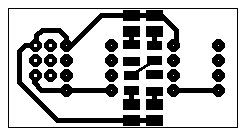
\includegraphics{sensorpcb.png}
\caption[Sensor pcb layout]{The pcb layout of the  sensor, not mirrored.}
\end{figure}

The layout was then mirrored and printed out onto thick glossy photo paper (Staples Photo Plus Gloss Paper to be exact) using a Brother laser printer with toner usage set to high. The Brother laser printer is all that I had on hand, an older model laser printer would have been ideal since the Brother laser printer toner have a high melting point, making it hard to melt the toner from the paper onto the copper. The glossy paper was then placed onto the copper board and ironed with a standard household clothes iron set to high. The iron was left on for about 15 minutes. After which, the iron was removed and the copper board placed into water to separate the paper from it. After about 10 minutes, the remaining paper was peeled off of the copper board by hand. 

The toner was now stuck to the copper board. Any broken traces were touched up with a Sharpie marker. The opposite side (the ground plane) was coloured black to prevent the enchant from eating away at it. The board was then submerged in the etching solution (Ferric Chloride) to remove the exposed copper. After about 20 minutes, the exposed copper was removed and the board fully etched. The board was then rinsed off in water and cleaned up with acetone to remove the toner and Sharpie marker from the board. Any extra copper traces were scraped off. Solder was placed onto the copper traces to prevent oxidation and make soldering the components easier. The PCB was then complete as can be seen in Figure 4.7.

\begin{figure}[htp]
\centering
\subfigure[Sensor after etching]{ 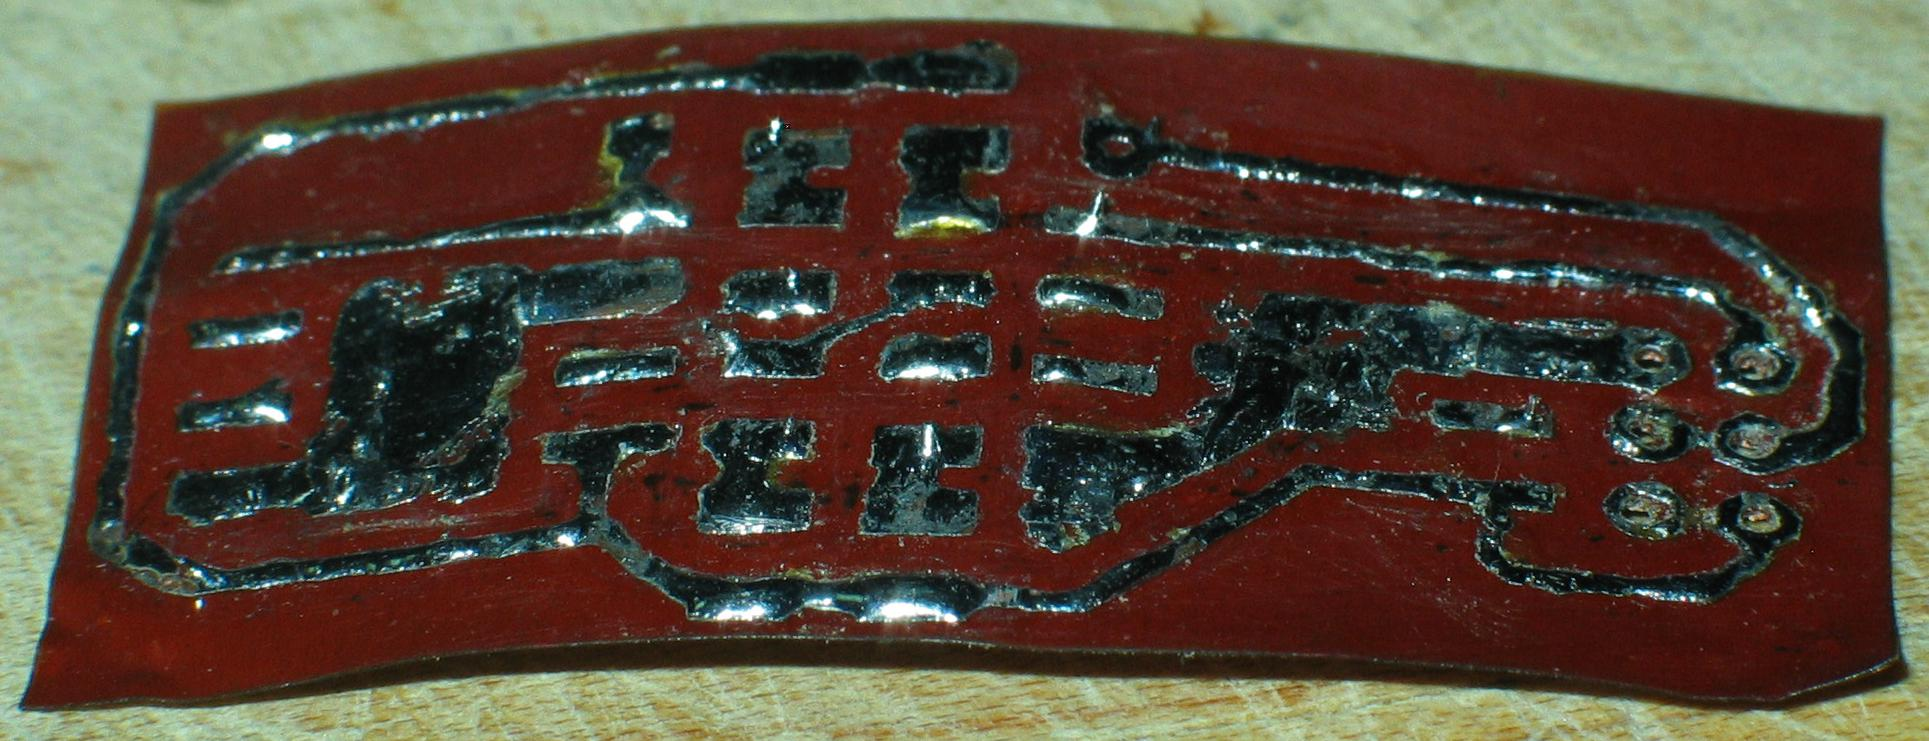
\includegraphics[width=6in]{sensorproto.jpg}}
\subfigure[Sensor showing flexibility]{ 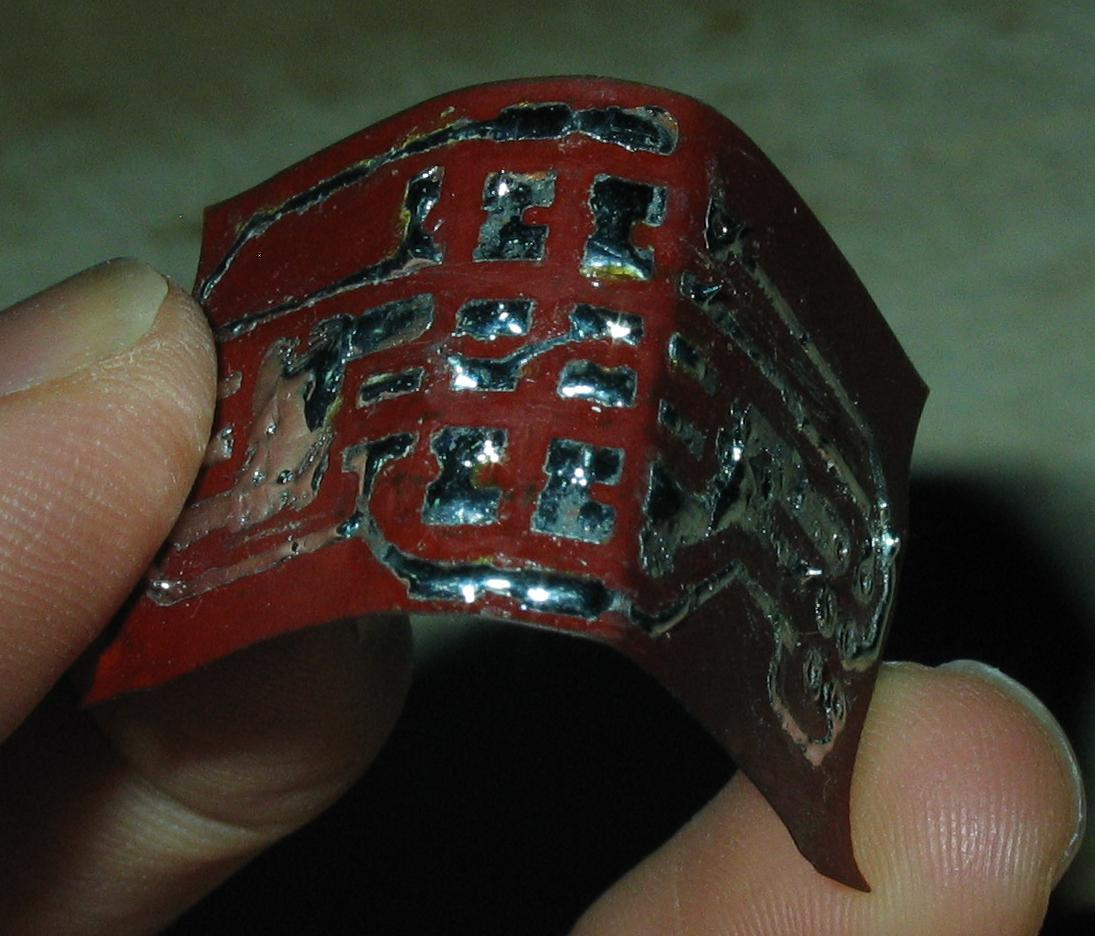
\includegraphics[width=6in]{sensorbend.jpg}}
\caption[Sensor prototype PCB]{The completed sensor PCB}
\end{figure}

Unfortunately, I made the traces to thin. While the came out okay out of the etchant, after many bends, some traces broke (even though they appeared fine). 

Again, the majority of the electrical components were obtained from Digikey. With the exception of the OPT101 monolithic photodiode, which was obtained from Texas Instruments as a free sample. After populating the sensor and difficult task of adding jumper wires, the finalized sensor prototype was complete. Correctly building the board took quite a few hours to complete. The complete sensor can be seen in Figure 4.8. Due to time constraints only 1 sensor was built. Though, the microcontroller was designed to handle 2.

\begin{figure}[htp]
\centering
\subfigure[Complete Sensor Prototype]{ 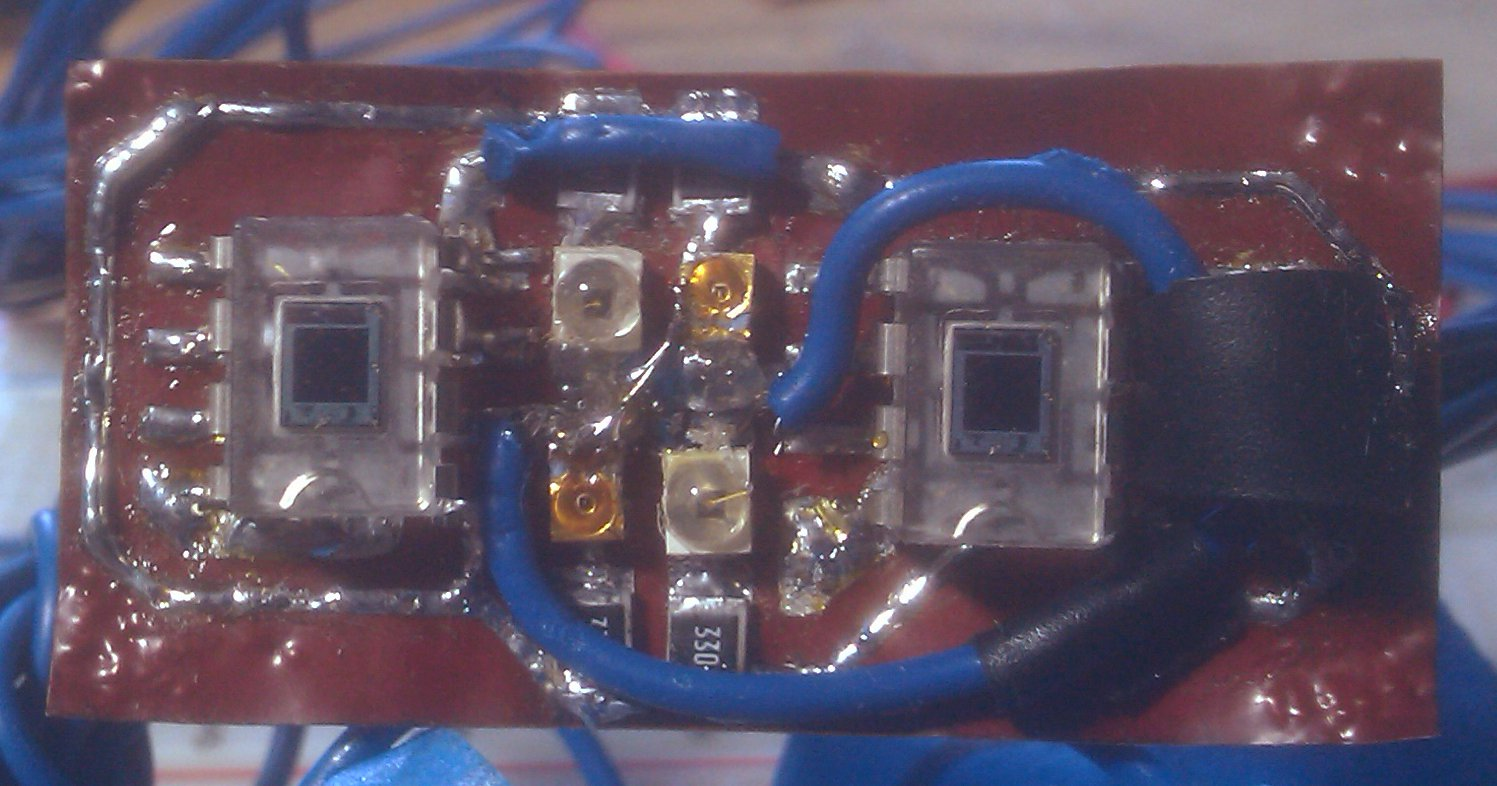
\includegraphics[width=6in]{csensorproto.jpg}}
\subfigure[Sensor Prototype showing flexibility]{ 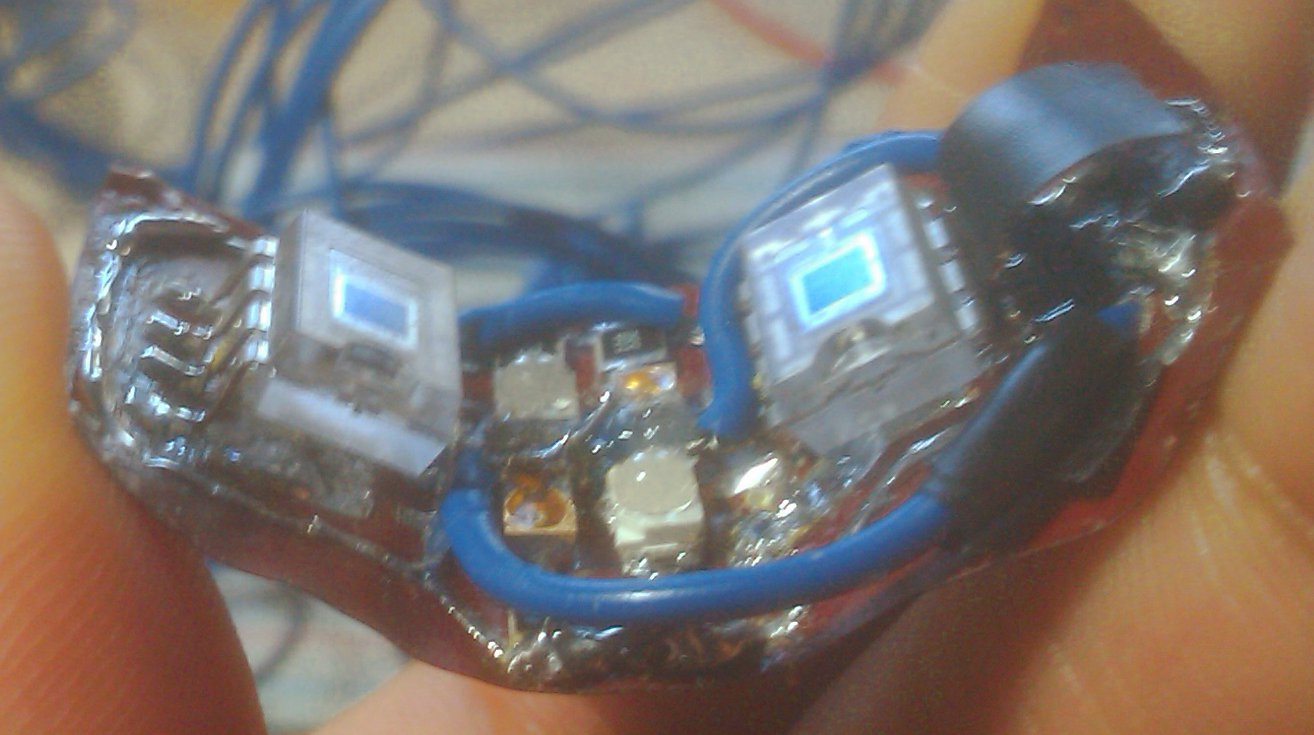
\includegraphics[width=6in]{csensorbend.jpg}}
\caption[Finalized Sensor Prototype]{The finalized complete sensor}
\end{figure}

\section{Software}

To write the software for the microcontroller, C was selected over assembly to reduce development time and increase readability. As discussed above, the UART function had to be written in software in addition to data acquisition. To do this, example timer UART code by L. Westlund at Texas Instruments, available in the IAR Embedded Workbench example files, was used as a basis for the software UART functionality. This was done because the author did not know how to implement the UART functionality from scratch. Once UART was working, data acquisition was tackled.

\subsection{Data Acquisition}
Due to the slow haemodynamic response in your brain due to activity, a time resolution of 10ms (or 100Hz) is all that is needed. That is all the wavelengths and positions must be sampled at least every 10 ms.

To do this, data is sampled in a time multiplexed fashion. That is, all the data is sampled independently in a certain order within the time resolution. 

Firstly the sensors are sampled with all the LEDs off to obtain the background light intensity. Then the first wavelength of LED is turned on and allowed to stabilize for a period of time. Then the first signal is obtained from the first OPT101 photodiode, subtracted by the background light intensity, and transmitted to the computer.  Then the second signal is obtained from the second OPT101 photodiode, subtracted by the background light intensity, and transmitted to the computer. Then the LEDs are turned off, the second wavelength LEDs turned on, allowed to stabilize, and the cycle repeated. Once this cycle is completed, all the LEDs are turned off, the background light intensity sampled, and the cycle repeats. This is illustrated in Figure 4.9. Though, perhaps it is more easily seen in the microcontroller code flow chart in Appendix B.1.

\begin{figure}[htp]
\centering
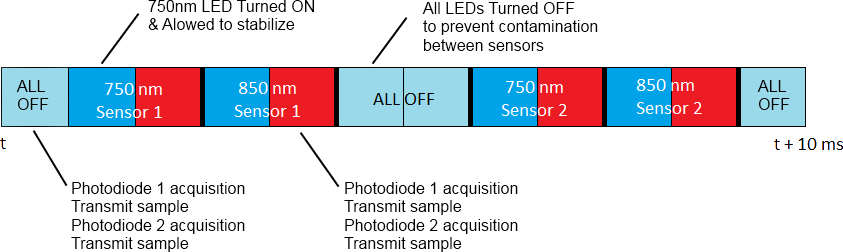
\includegraphics[width=6in]{data.png}
\caption[Time multiplexed acquisition]{An illustration of the time multiplexed acquisition cycle.}
\end{figure}

\subsection {Computer Software}

To write the software, Ruby was selected as the language of choice. It was selected due to the author's desire to learn Ruby as it is a very popular dynamic general purpose object-oriented programming language. It is spoken highly of by many experienced computer science veterans. While not up to the speed of C or C++, Ruby has amazingly good performance for a dynamic programming language.

The computer software must firstly obtain the data from the device. To do this the serialport library from rubygems (a host of many Ruby librarys or 'gems') was used to interact with the serial port on the computer, communicating through UART. The serial port is opened, sent the message 'S', to message the device to begin acquiring data. The program then receives the data. The data is split into two parts the upper 8 bit and the lower 8 bits when it is received. The program combines them together and divides the resulting value by 0xFFFF. The reason for this is the output from the ADC on the microcontroller is relative to its maximum value of 0xFFFF. To ensure the data arrives correctly, an 'S' is transmitted by the device before sending each set of data to ensure that the device is synchronized correctly with the computer. Once all the data is received, the calculations are done on the raw data to obtain the necessary relevant values.

Equations 3.7 and 3.8 were used to calculate the change in concentrations. Equation 3.6 was used to calculate the differential optical density. During the project demonstration Equation 3.6 was not written correctly in the code, giving wrong results. This has since been fixed and the differential optical density is now calculated correctly. In order to calculate the change in concentrations, first the specific wavelength constant and differential pathlength factors must be found.

Since the specific wavelength extinction coefficient of the absorber($\epsilon^\lambda$) cannot be directly measured with near infrared light, they are found by interpolating the values given for these coefficients for oxyhaemoglobin and deoxyhaemoglobin in literature, specifically \cite{wray88} and \cite{roe91}. This results in $\epsilon^{750nm}_Hb$ = 1.532, $\epsilon^{750nm}_O2Hb$ = 0.600, $\epsilon^{850nm}_Hb$ = 0.781, $\epsilon^{850nm}_O2Hb$ = 1.097. Calculating the differential pathlength factor (DPF$^\lambda$) yeilds $DPF^{730nm}$=5.0055 and $DPF^{850nm}$=4.6564. The calculation for DPF$^\lambda$ can be seen in Appendix A.2.

Once the calculations are complete the change in concentrations are output to text files that can be read by Matlab. The data is very noisy and requires a low pass filter to be done on it to obtain the necessary data. Due to time limitations, a low pass filter was not able to be made in Ruby for the software. As such, Matlab was decided to be used to filter the data. As per \cite{wolf05}, a low pass filter with a cutoff of 0.5Hz should be used. Therefore a low pass fourth-order butterworth filter was used with a cutoff of 0.5Hz. The Matlab source code can be seen in Appendix C. Taking the Fourier transform of the data before filtering gives the result in Figure 4.10(a). Taking the Fourier transform of the data after filtering gives the result in Figure 4.10(b).

\begin{figure}[htp]
\centering
\subfigure[FFT of data before filtering]{ 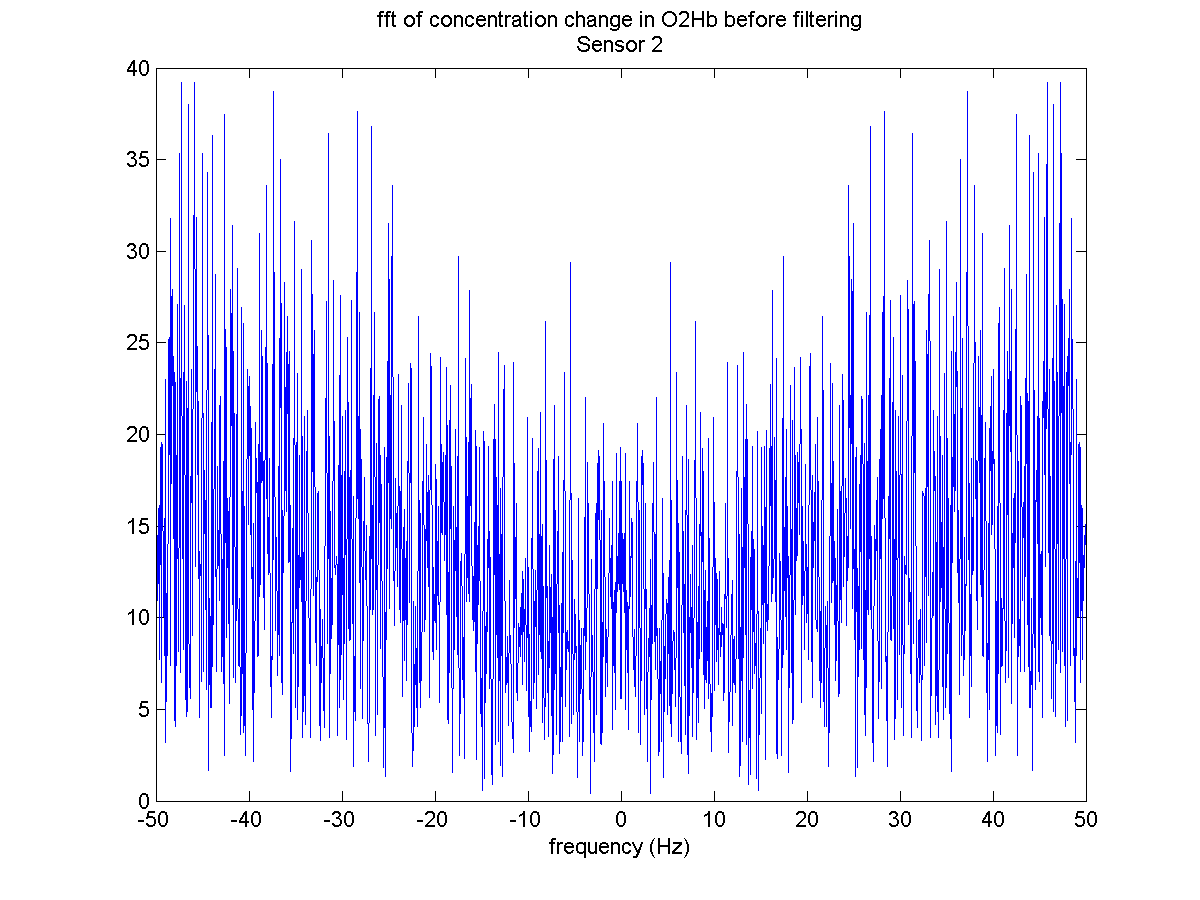
\includegraphics[width=4in]{fftHbO2_2.png}}
\subfigure[FFT of data after filtering]{ 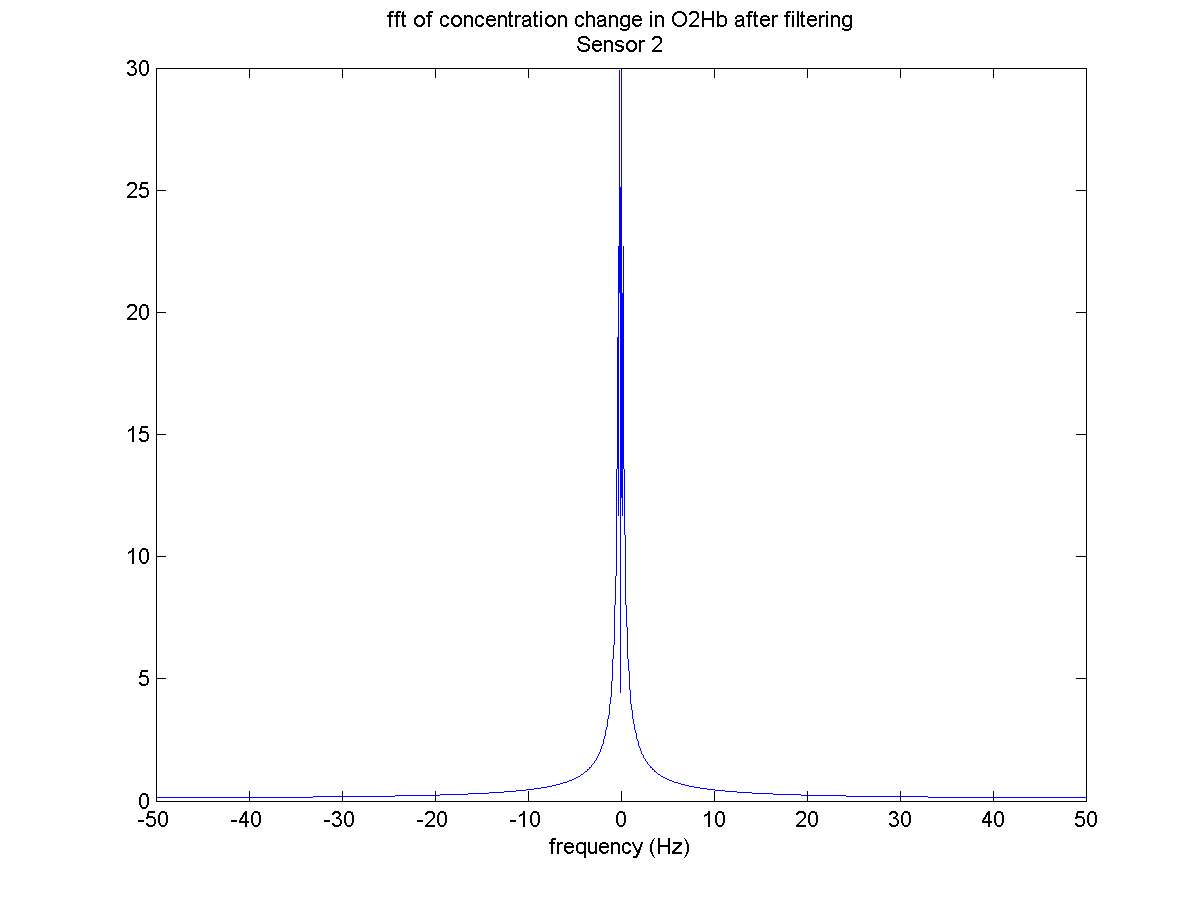
\includegraphics[width=4in]{fftHbO2_2f.png}}
\caption[FFT of data]{The FFT of the data before filtering and after filtering. The data used is the change in oxyhaemoglobin during motor movement}
\end{figure}

The design of the device is now complete and results can be seen.

\section{Cost}

Since one of the goals of this project is to low-cost, Table 4.1 shows the total cost to build one of these systems with one sensor. The USB to UART module will be left out since it is only needed for programming the device. In a mass produced system, the microcontroller would be programmed by JTAG anyway.

\begin{table}
  \caption{Cost of 1 NIRS System}
  \begin{tabular}{| l | c | r | r |}
\hline
\multicolumn{4}{|c|}{Cost of 1 NIRS System} \\
\hline
\bf Item & \bf Quantity & \bf Unit Price & \bf Total Price \\ \hline
LDO Regulator&1&\$1.85&\$1.85\\
1$\mu$f Capacitors&4&\$0.05&\$0.20\\
0.01$\mu$f Capacitors&4&\$0.01&\$0.04\\
32KHz Crystal&1&\$0.36&\$0.36\\
MSP430f4250&1&\$4.55&\$4.55\\
Power LED&1&\$0.10&\$0.10\\
330$\Omega$ Resistor&2&\$0.06&\$0.12\\
Bluetooth LED&1&\$0.12&\$0.12\\
Bluetooth module&1&\$18.00&\$18.00\\
SPDT Switch&1&\$3.99&\$3.99\\
2N4401 BJT&2&\$0.14&\$0.28\\ \hline
\multicolumn{3}{|r}{\em Subtotal}&\$29.61 \\ \hline
\multicolumn{4}{|l|}{\bf Sensor} \\ \hline
750nm LED&2&\$3.02&6.04\\
850nm LED&2&\$1.17&\$2.34\\
33$\Omega$ Resistor&4&\$0.17&\$0.68\\
OPT101 Photodiode&2&\$6.23&\$12.46\\ \hline
\multicolumn{3}{|r}{\em Subtotal}&\$21.52 \\ 
\multicolumn{3}{|r}{\bf \em Total}&\bf \$51.13 \\
\hline
  \end{tabular}
\end{table}

\section{Design Challenges}
The initial design challenges encountered were sourcing the LEDs. A consumer retailer could not be found selling LEDs of a wavelength between 700nm - 830nm. Many email had to be sent out to various manufacturers, retailers, and distributors until the Marubeni Corporation responded that they would be willing to sell some samples.

The Majority of the other design challenges stem from the author's inexperience with microcontroller design and time constraints. 

Perhaps one of the longest challenges that had to be overcome was the UART communication. After the prototype was built, it would not communicate over UART via the USB to UART module. After much troubleshooting and going over the design many times, comparing my circuit design to another MSP430 project that used UART, it was determined that the TX and RX wires were swapped. Originally the TX output from the USB UART module was connected to the TX output of the microcontroller and the RX input connected to the RX input. Due to inexperience, the author believed that the connection matched up rather than the logical way of TX to RX.

Now that the bootloader was able to be programmed, implementing the software timer UART was a daunting task. Writing custom code proved to be futile, so example code was turned to for the UART implementation. However, even unmodified sample code was not communicating to the computer. Code was executing correctly on the device, it was possible to to flash LEDs and such. However, once a serial terminal was opened on the computer, code would stop executing, as if it was stuck in an interrupt. Due to the decision to not use a JTAG programmer, debugging could only be done via LEDs. 

After many countless hours, it was realized that the DTR line on the USB UART module was setting RST to low on the microcontroller, resetting the device. The RST wire is there because it is needed to invoke the bootloader and is part of the flow control used by the built-in bootloader. However, it must be disconnected when not trying to invoke the bootloader.

The flexible sensor provided a great design challenge. If the  creation of the sensor was not difficult enough, populating the board was. Due to the decision to make the sensor as small as possible and being only a single sided SMD PCB, jumper wires were used to connect certain components. This made it a large pain to solder the components. Additionally, small traces were selected. Had the board been ridged rather than flexible, this design would have been fine since the traces came out okay. But after many bends and flexes, some of the traces broke, even if they appeared to be okay. These were easily fixable by soldering the traces back together. However, it provided a big headache when testing the device.

The computer software also played a somewhat large challenge and is perhaps the weakest part of this project and the main reason for its poor performance. Data acquisition played a problem at first. The microcontroller and computer were not in sync, and the computer received many null data points when trying to retrieve the data. However after properly matching the times between the two programs through the use of sleep functions, the data was retrieved correctly. The switch to the Bluetooth module removed these errors, everything synced up fine and the sleep functions code be removed. It is assumed that there are performance issues with the FTDI USB UART driver in Linux. However, the microcontroller still sends the char 'S' before each measurement to ensure everything syncs up fine.